\documentclass[
aspectratio=169 % comment for 4:3
]{beamer}
\usepackage{tabularx}

\newcommand{\cmd}[1]{\texttt{\textbf{#1}}}
\newcommand{\args}[1]{\texttt{\textit{#1}}}

\usetheme[
hidetotal, % hide the total number of slides on the bottom right
hidenumbers, % hide current slide number
% hidename, % hide author name and title in footline
hidebullets, % use empty bullets in itemize
hidefootline, % hide the footline
%
% the previous options allow for a minimalistic style as recommended by Patrick
% Winston in his "how to speak" lecture at MIT
%
% sidebar, % show sidebar
hugetitle, % print main title in huge font
% thin, % use a thinner font
% bold, % use bold titles
% standardtitle, % use standard title slide (no picture)
]{mfrancois}

\setsecondarylogo{title/isia-logo} % Add a secondary logo to the title slide, optional
\settitleimage{title/raspberry} % Change the title slide image, optional (use images with a ratio identical to the one provided)

\author[F. Marelli]{François Marelli}
\affiliation[UMONS]{UMONS, ISIA Lab}
\title{Atelier Créactifs: Raspberry Pi}
\subtitle{Séance 6: Partage de fichiers et serveur multimédia}
\extras{
\includegraphics[height=25pt]{title/creactifs}}
\date{23 mars 2026}

\graphicspath{{images}}

\begin{document}

\maketitle

\begin{frame}{Avant de commencer}{Désactiver les services}

    \begin{enumerate}
        \item Vérifier l'état des services de la séance précédente:

              \cmd{sudo systemctl}\args{ status mediamtx}

              \cmd{systemctl}\args{ -{}-user status homeassistant}

        \item Si nécessaire, les arrêter:

              \cmd{sudo systemctl}\args{ stop mediamtx}

              \cmd{systemctl}\args{ -{}-user stop homeassistant}
        \item Et désactiver leur démarrage automatique:

              \cmd{sudo systemctl}\args{ disable mediamtx}

              %\begin{noindent}
              \cmd{rm}\args{
                  \textasciitilde/.config/containers/systemd/homeassistant.container}
              %\end{noindent}

    \end{enumerate}

\end{frame}

\begin{frame}{Partage de fichiers à distance}

    Samba:
    \begin{itemize}
        \item Logiciel de partage de fichiers
        \item Compatible Linux, Windows, macOS
        \item Dossier partagé accessible via le réseau local
    \end{itemize}

    \bigskip
    \(\rightarrow\) le dossier partagé est comme une "clé USB" accessible à
    distance

    \medskip
    \(\rightarrow\) serveur "cloud" local (comme Google Drive, OneDrive,
    Dropbox)

\end{frame}

\begin{frame}{Configurer samba}
    Les ingrédients:
    \begin{enumerate}
        \item Le logiciel Samba
        \item Un dossier à partager
        \item Un fichier de configuration pour Samba
        \item Un utilisateur Samba
    \end{enumerate}
\end{frame}

\begin{frame}{Configurer samba}{1. Installer le logiciel Samba}
    \cmd{sudo apt install}\args{ samba}

    \bigskip
    On commence à connaître
\end{frame}

\begin{frame}{Configurer samba}{2. Créer un dossier à partager}
    \cmd{mkdir}\args{ \textasciitilde/partage}

    \bigskip
    \(\rightarrow\) Seul l'intérieur de ce dossier sera accessible via Samba

    \bigskip
    \alert{Attention:} pour un cas d'usage réel, il faut éviter de partager un
    dossier sur la carte SD, préférer un disque externe pour la durabilité
\end{frame}

\begin{frame}[fragile]{Configurer samba}{3. Écrire un fichier de configuration}
    \cmd{sudo nano}\args{ /etc/samba/smb.conf}

    \bigskip
    Ajouter à la fin du fichier:

    \begin{verbatim}
    [partage]
    path = /home/rpi/partage
    writeable = yes
    browseable = yes
    public = no
    \end{verbatim}

    Options pour définir le nom, le chemin, les permissions (écriture,
    visibilité) et la sécurité
\end{frame}

\begin{frame}{Configurer samba}{4. Créer un utilisateur Samba}
    \cmd{sudo smbpasswd}\args{ -a rpi}

    (utiliser \texttt{rpi} comme mot de passe)

    \bigskip
    \(\rightarrow\) L'utilisateur \texttt{rpi} est autorisé à accéder au
    partage Samba avec le mot de passe défini

    \bigskip
    \bigskip
    Appliquer les changements en redémarrant le service Samba:

    \cmd{sudo systemctl}\args{ restart smbd}
\end{frame}

\begin{frame}[fragile]{Se connecter à un serveur Samba}

    Depuis Linux ou macOS, ajouter le serveur:

    \begin{verbatim}smb://adresse_ip/partage\end{verbatim}

    \bigskip
    Depuis Windows, ajouter un lecteur réseau:

    \begin{verbatim}\\adresse_ip\partage\end{verbatim}

    \bigskip
    \alert{Attention:} il faut utiliser l'utilisateur Samba et non son
    identifiant local

    \bigskip
    \textbf{Exercice:} créer un fichier texte dans le dossier partagé depuis
    votre ordinateur et l'afficher sur la Raspberry Pi

\end{frame}

\begin{frame}{Kodi}{Transformer tout en Smart TV}
    \begin{columns}
        \begin{column}{.3\textwidth}
            \centering
            
\includegraphics[width=\textwidth]{kodi}

        \end{column}
        \begin{column}{.7\textwidth}
            Kodi:
            \begin{itemize}
                \item Logiciel open source
                \item Interface pour la lecture de vidéos, musique, photos
                \item Compatible avec de nombreux formats et services
                \item Contrôlable avec la télécommande
            \end{itemize}

        \end{column}
    \end{columns}
    \bigskip
    \(\rightarrow\) Permet de transformer la Raspberry Pi en lecteur
    multimédia
\end{frame}

\begin{frame}{Kodi}{Transformer tout en Smart TV}
    \centering
    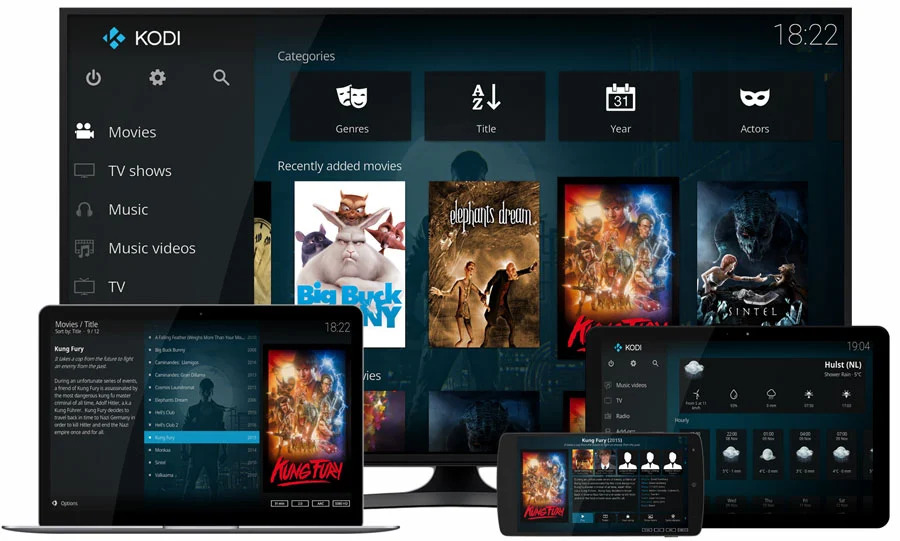
\includegraphics[width=.7\textwidth]{kodi_screen}
\end{frame}

\begin{frame}{Installer Kodi}
    Plusieurs options:
    \begin{itemize}
        \item OS dédié: LibreELEC, OSMC
        \item \alert{En tant que logiciel}
    \end{itemize}

    \bigskip
    \cmd{sudo apt}\args{ install kodi}

    \bigskip
    Lancer dans le terminal avec \cmd{kodi} ou depuis le menu

    \bigskip
    \alert{Tip:} Kodi peut être contrôlé depuis Home Assistant!

\end{frame}

\begin{frame}{Jellyfin}{Votre propre Netflix}
    \begin{columns}
        \begin{column}{.3\textwidth}
            \centering
            
\includegraphics[width=\textwidth]{jellyfin}

        \end{column}
        \begin{column}{.7\textwidth}
            Jellyfin:
            \begin{itemize}
                \item Serveur de médias open source
                \item Organise et diffuse votre collection de médias
                \item Accès à distance via une interface web ou des applications
            \end{itemize}

            \bigskip
            Kodi: lecteur, Jellyfin: source

            \bigskip
            \url{https://demo.jellyfin.org}
        \end{column}
    \end{columns}

\end{frame}

\begin{frame}[fragile]{Jellyfin}{Installation}
    Pas assez de RAM sur la Raspberry Pi 3 pour l'installation standard

    \bigskip
    \(\rightarrow\) Utiliser un conteneur:

    \begin{verbatim}
    podman pull docker.io/jellyfin/jellyfin:latest
    \end{verbatim}

\end{frame}

\begin{frame}[fragile]{Jellyfin}{Lancement}

    \begin{lstlisting}[language={}]
    podman run \
        --detach \
        --label "io.containers.autoupdate=registry" \
        --name jellyfin \
        --publish 8096:8096/tcp \
        --publish 7359:7359/udp \
        --rm \
        --user $(id -u):$(id -g) \
        --userns keep-id \
        --volume jellyfin-cache:/cache:Z \
        --volume jellyfin-config:/config:Z \
        --mount type=bind,source=/home/rpi,destination=/media,ro=true,relabel=private \
        docker.io/jellyfin/jellyfin:latest
    \end{lstlisting}
\end{frame}

\begin{frame}[fragile]{Jellyfin}{Interface web}

    Accéder à l'interface web de Jellyfin:

    \begin{verbatim}
    http://adresse_ip:8096
    \end{verbatim}

    \bigskip
    Créer un compte utilisateur et découvrir l'interface

    \bigskip
    \alert{Tip:} le serveur Jellyfin est accessible depuis n'importe quel
    appareil du réseau local!

\end{frame}

\begin{frame}{Exercice final}{Combiner Kodi et Jellyfin}

    Par groupe de 2 machines:
    \begin{enumerate}
        \item Lancer un serveur Jellyfin sur une machine
        \item Lancer Kodi sur l'autre machine
        \item Installer un add-on Kodi pour se connecter à Jellyfin
    \end{enumerate}

    \bigskip
    Objectif: lire un média à distance

\end{frame}

\end{document}
